%%%%%%%%%%%%%%%%%%%%%%%%%%%%%%%%%%%%%%%%%%%%%%%%%%%%%%%%%%%%%%%%%%%%%%
%     File: ExtendedAbstract_resul.tex                               %
%     Tex Master: ExtendedAbstract.tex                               %
%                                                                    %
%     Author: Andre Calado Marta                                     %
%     Last modified : 27 Dez 2011                                    %
%%%%%%%%%%%%%%%%%%%%%%%%%%%%%%%%%%%%%%%%%%%%%%%%%%%%%%%%%%%%%%%%%%%%%%
% Results
% Results should be clear and concise.
% Discussion
% This should explore the significance of the results of the work, not
% repeat them. A combined Results and Discussion section is often
% appropriate. Avoid extensive citations and discussion of published
% literature.
%%%%%%%%%%%%%%%%%%%%%%%%%%%%%%%%%%%%%%%%%%%%%%%%%%%%%%%%%%%%%%%%%%%%%%

\section{Results}
\label{sec:resul}

%- Cutflow table \\
%- ...

\begin{figure}[h]
	\centering
	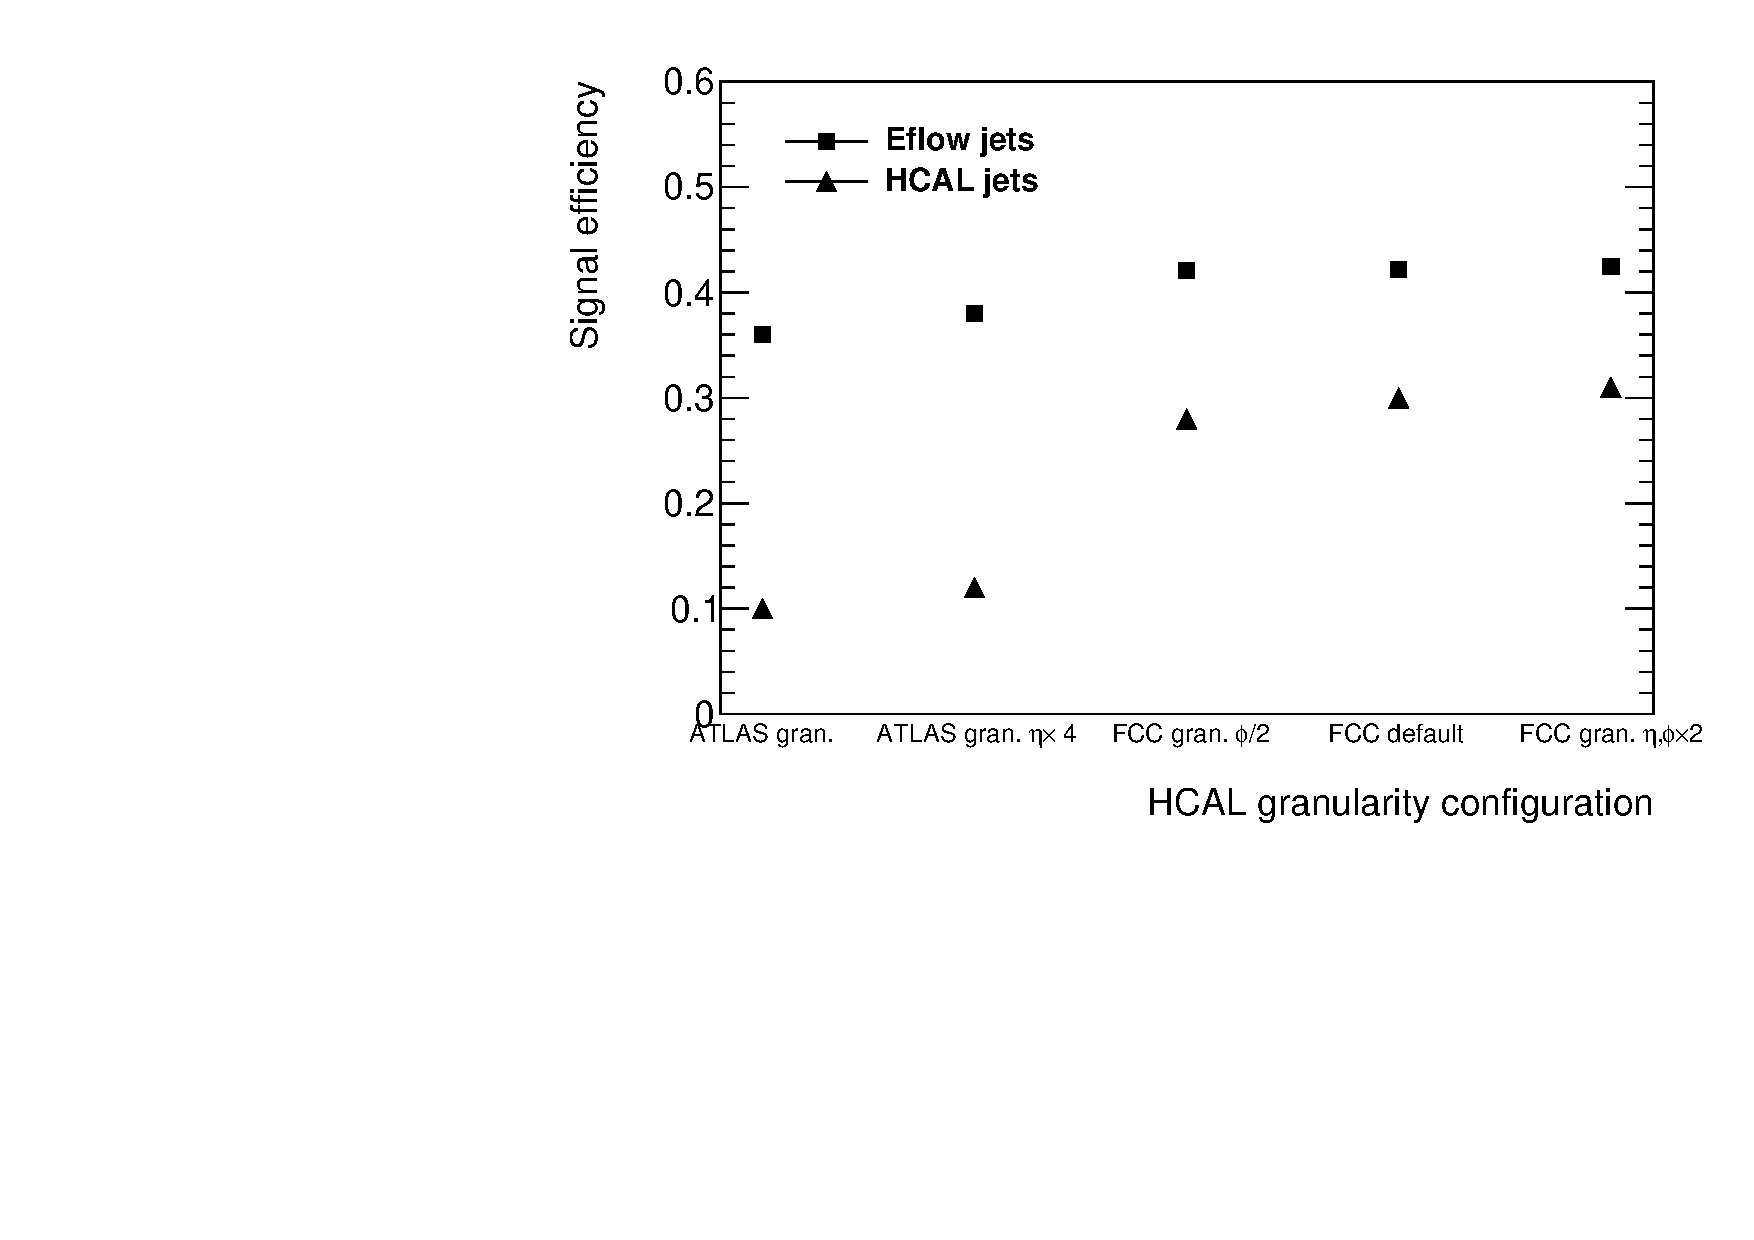
\includegraphics[width=\linewidth]{./images/EffPlotGran.pdf}
	\label{fig:eff_gran}
	\caption{oi}
\end{figure}

\begin{figure}[h]
	\centering
	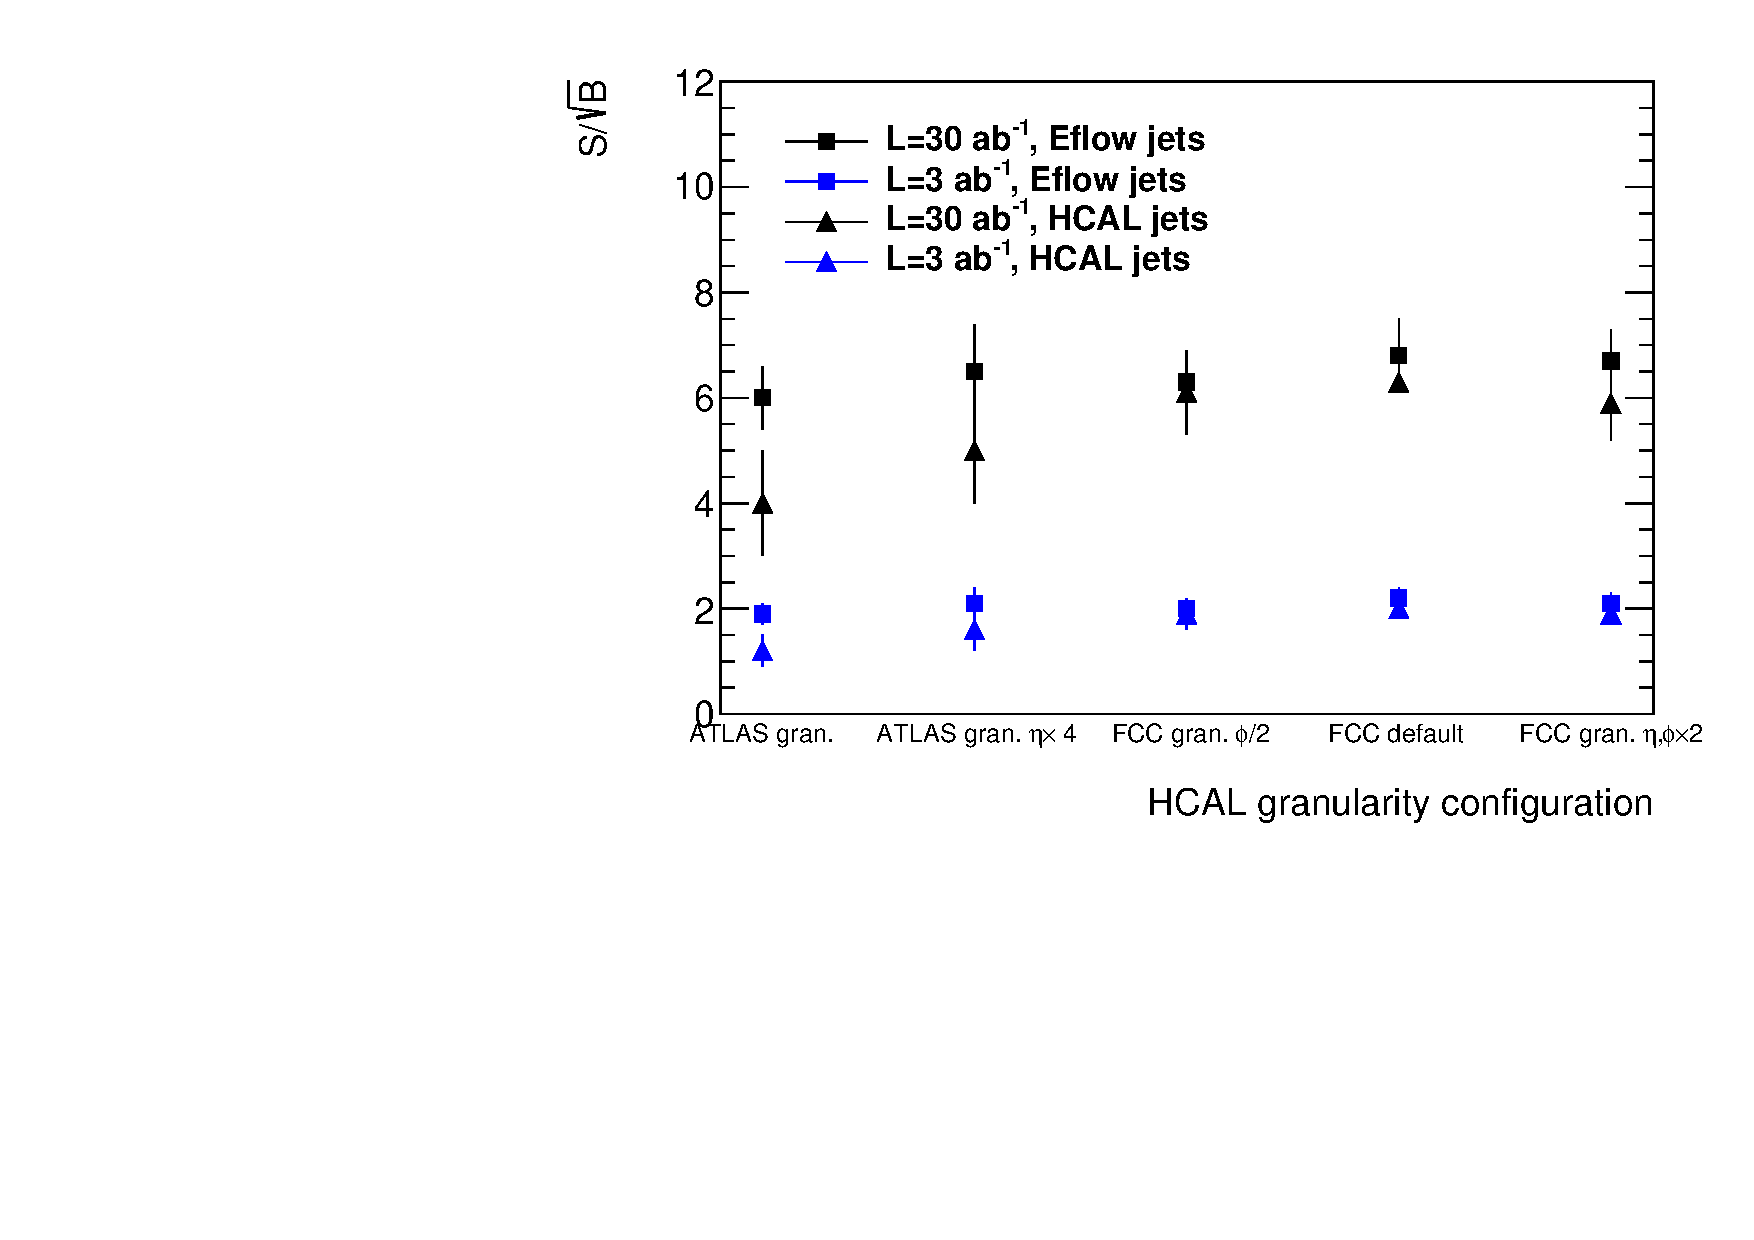
\includegraphics[width=\linewidth]{./images/SSBplotGran.pdf}
	\label{fig:SSB_gran}
	\caption{oi}
\end{figure}

